\section{Einleitung}\raggedbottom 

\subsection{Motivation und Zielsetzung} 
%Gallia est omnis divisa in partes tres,
%quarum unam
%incolunt Belgae, aliam Aquitani, tertiam qui ipsorum lingua
%Celtae, nostra Galli appellantur. Hi omnes lingua, institutis,
%legibus inter se differunt. Gallos ab Aquitanis Garumna flumen, a
%Belgis Matrona et Sequana dividit. Horum omnium fortissimi sunt
%Belgae, propterea quod a cultu atque humanitate provinciae
%longissime absunt, minimeque ad eos mercatores saepe commeant
%atque ea quae ad effeminandos animos pertinent important,
%proximique sunt Germanis, qui trans Rhenum incolunt, quibuscum
%continenter bellum gerunt. Qua de causa Helvetii quoque reliquos
%Gallos virtute praecedunt, quod fere cotidianis proeliis cum
%Germanis contendunt, cum aut suis finibus eos prohibent aut ipsi
%in eorum finibus bellum gerunt. Eorum una, pars, quam Gallos
%obtinere dictum est, initium capit a flumine Rhodano, continetur
%Garumna flumine, Oceano, finibus Belgarum, attingit etiam ab
%Sequanis et Helvetiis flumen Rhenum, vergit ad septentriones.
%Belgae ab extremis Galliae finibus oriuntur, pertinent ad
%inferiorem partem fluminis Rheni, spectant in septentrionem et
%orientem solem. Aquitania a Garumna flumine ad Pyrenaeos montes et
%eam partem Oceani quae est ad Hispaniam pertinet; spectat inter
%occasum solis et septentriones.


\subsection{Vorgehensweise}
%Apud Helvetios longe nobilissimus fuit et
%ditissimus
%Orgetorix. Is M. Messala, [et P.] M. Pisone consulibus regni
%cupiditate inductus coniurationem nobilitatis fecit et civitati
%persuasit ut de finibus suis cum omnibus copiis exirent: perfacile
%esse, cum virtute omnibus praestarent, totius Galliae imperio
%potiri. Id hoc facilius iis persuasit, quod undique loci natura
%Helvetii continentur: una ex parte flumine Rheno latissimo atque
%altissimo, qui agrum Helvetium a Germanis dividit; altera ex parte
%monte Iura altissimo, qui est inter Sequanos et Helvetios; tertia
%lacu Lemanno et flumine Rhodano, qui provinciam nostram ab
%Helvetiis dividit. His rebus fiebat ut et minus late vagarentur et
%minus facile finitimis bellum inferre possent; qua ex parte
%homines bellandi cupidi magno dolore adficiebantur. Pro
%multitudine autem hominum et pro gloria belli atque fortitudinis
%angustos se fines habere arbitrabantur, qui in longitudinem milia
%passuum CCXL, in latitudinem CLXXX patebant.
%
%His rebus adducti et auctoritate Orgetorigis permoti constituerunt
%ea quae ad proficiscendum pertinerent comparare, iumentorum et
%carrorum quam maximum numerum coemere, sementes quam maximas
%facere, ut in itinere copia frumenti suppeteret, cum proximis
%civitatibus pacem et amicitiam confirmare. Ad eas res conficiendas
%biennium sibi satis esse duxerunt; in tertium annum profectionem
%lege confirmant. Ad eas res conficiendas Orgetorix deligitur. Is
%sibi legationem ad civitates suscipit. In eo itinere persuadet
%Castico, Catamantaloedis filio, Sequano, cuius pater regnum in
%Sequanis multos annos obtinuerat et a senatu populi Romani amicus
%appellatus erat, ut regnum in civitate sua occuparet, quod pater
%ante habuerit; itemque Dumnorigi Haeduo, fratri Diviciaci, qui eo
%tempore principatum in civitate obtinebat ac maxime plebi acceptus
%erat, ut idem conaretur persuadet eique filiam suam in matrimonium
%dat. Perfacile factu esse illis probat conata perficere, propterea
%quod ipse suae civitatis imperium obtenturus esset: non esse
%dubium quin totius Galliae plurimum Helvetii possent; se suis
%copiis suoque exercitu illis regna conciliaturum confirmat. Hac
%oratione adducti inter se fidem et ius iurandum dant et regno
%occupato per tres potentissimos ac firmissimos populos totius
%Galliae sese potiri posse sperant. (siehe \cite{Con97},
%\cite{PeHe97} und Abbildung \ref{fig_Gallien})
%
%
%\begin{figure}[htb]
%\begin{center}
%  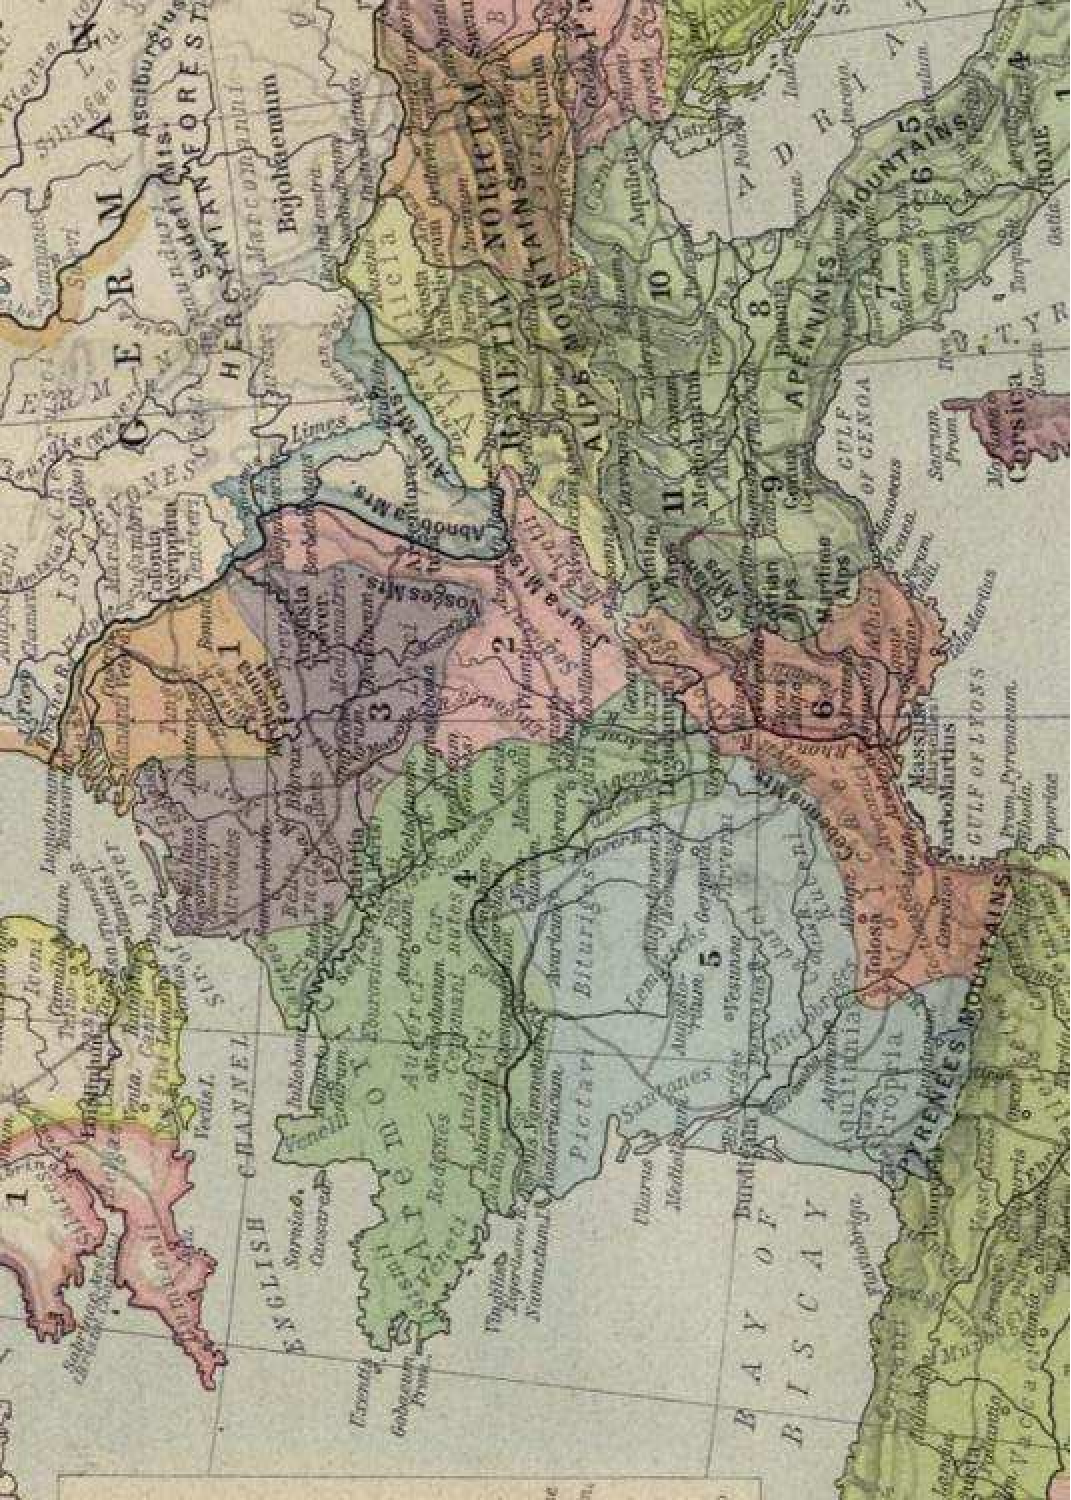
\includegraphics[width=175pt, angle=270]{bilder/Galia}
%  \caption{Gallien zur Zeit Caesars}\label{fig_Gallien}
%\end{center}
%\end{figure}
%
%
%\begin{table}[htb]
%\begin{center}
%\begin{tabular}{|l|l|l|}
%\hline
%Jahr &  Erster Consul & Zweiter Consul\\
%\hline \hline
%1 & C. Caesar         & L. Aemilius Paullus\\
%2 & P. Vinicius       & P. Alfenus Varus\\
%3 & L. Aelius Lamia   & M. Servilius\\
%4 & Sex. Aelius Catus &  C. Sentius Saturninus\\
%5 & L. Valerius Messalla& Cn. Cornelius Cinna \\
%suff. & C. Vibius Postumus &  C. Ateius Capito\\
%6 & M. Aemilius Lepidus & L. Arruntius\\
%\hline
%\end{tabular}
% \caption{Römische Konsulen}\label{tab_Konsulen}
%\end{center}
%\end{table}


\pagebreak

\section{Definitionen und Grundlagen}\raggedbottom
\subsection{Das formale Problem}
\subsection{Evaluation}
\subsection{Die Daten}

%Pharnace superato, Africa recepta, qui ex his proeliis cum
%adulescente Cn. Pompeio profugissent, cum . . . et ulterioris
%Hispaniae potitus esset, dum Caesar muneribus dandis in Italia
%detinetur, . . . quo facilius praesidia contra compararet,
%Pompeius in fidem uniuscuiusque civitatis confugere coepit. Ita
%partim precibus partim vi bene magna comparata manu provinciam
%vastare. Quibus in rebus non nullae civitates sua sponte auxilia
%mittebant, item non nullae portas contra cludebant. Ex quibus si
%qua oppida vi ceperat, cum aliquis ex ea civitate optime de Cn.
%Pompeio meritus civis esset, propter pecuniae magnitudinem alia
%qua ei inferebatur causa, ut eo de medio sublato ex eius pecunia
%latronum largitio fieret. Ita pacis commoda hoste +hortato+
%maiores augebantur copiae. +Hoc crebris nuntiis in Italiam missis
%civitates contrariae Pompeio+ auxilia sibi depostulabant.
%
%C. Caesar dictator tertio, designatus dictator quarto multis
%+iterante diebus coniectis+ cum celeri festinatione ad bellum
%conficiendum in Hispaniam cum venisset, legatique Cordubenses, qui
%a Cn. Pompelo discessissent, Caesari obviam venissent, a quibus
%nuntiabatur nocturno tempore oppidum Cordubam capi posse, quod nec
%opinantibus adversariis eius provinciae potitus esset, simulque
%quod tabellariis, qui a Cn. Pompeio dispositi omnibus locis
%essent, qui certiorem Cn. Pompeium de Caesaris adventu facerent .
%. . multa praeterea veri similia proponebant. Quibus rebus
%adductus quos legatos ante exercitui praefecerat Q. Pedium et Q.
%Fabium Maximum de suo adventu facit certiores, utque sibi
%equitatus qui ex provincia fuisset praesidio esset. Ad quos
%celerius quam ipsi opinati sunt appropinquavit neque, ut ipse
%voluit, equitatum sibi praesidio habuit.
%
%Erat idem temporis Sex. Pompeius frater qui cum praesidio Cordubam
%tenebat, quod eius provinciae caput esse existimabatur; ipse autem
%Cn. Pompeius adulescens Uliam oppidum oppugnabat et fere iam
%aliquot mensibus ibi detinebatur. Quo ex oppido cognito Caesaris
%adventu legati clam praesidia Cn. Pompei Caesarem cum adissent,
%petere coeperunt uti sibi primo quoque tempore subsidium mitteret.
%Caesar - eam civitatem omni tempore optime de populo Romano
%meritam esse - celeriter sex cohortis secunda vigilia iubet
%proficisci, pari equites numero. Quibus praefecit hominem eius
%provinciae notum et non parum scientem, L. Vibiurn Paciaecum. Qui
%cum ad Cn. P praesidia venisset, incidit idem temporis ut
%tempestate adversa vehementique vento adflictaretur; aditusque vis
%tempestatis ita obscurabat ut vix proximum agnoscere possent.
%Cuius incommodum summam utilitatem ipsis praebebat. Ita cum ad eum
%locum venerunt, iubet binos equites conscendere, et recta per
%adversariorum praesidia ad oppidum contendunt. Mediisque eorum
%praesidiis cum essent, cum quaereretur qui essent unus ex nostris
%respondit, ut sileat verbum facere: nam id temporis conari ad
%murum accedere, ut oppidum capiant; et partim tempestate impediti
%vigiles non poterant diligentiam praestare, partim illo responso
%deterrebantur. Cum ad portam appropinquassent, signo dato ab
%oppidanis sunt reccepti, et pedites dispositi partim ibi
%remanserunt, equites clamore facto eruptionem in adversariorum
%castra fecerunt.

\pagebreak
\section{Lösungsstrategien}\raggedbottom 
\subsection{Eigene Ansätze}
\subsubsection{Logstic Regression}
\subsubsection{k-Nearest-Neighbours}
\subsection{Neural Networks}
\subsection{Regularized Greedy Forest}
\subsection{XGBoost}